\begin{figure}
    \centering
    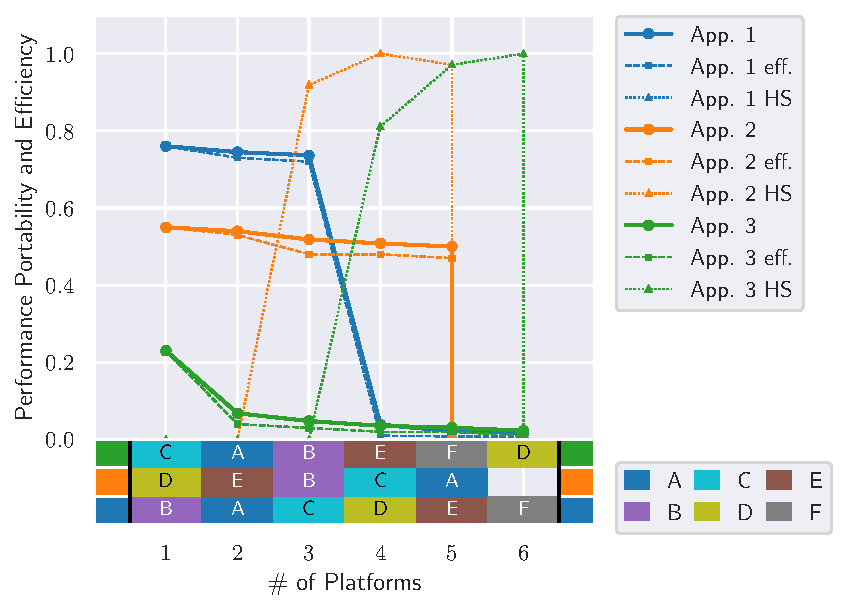
\includegraphics[width=\linewidth]{figures/02_performance_portability/example_diss_eff_cascade_with_HS.pdf}
    \caption{%
    An example visualization of the architectural efficiencies of \autoref{tab:example_effs} and performance portability scores of \autoref{tab:example_pp} of the three example applications as proposed by \citet{sewall_interpreting_2020}. 
    This time, the newly proposed heterogeneity score $HS$ (\autoref{def:hetero_score}) is added using dotted lines. 
    }
    \label{fig:vis_example_pp_hs}
\end{figure}

\autoref{fig:vis_example_pp_hs} displays the same plot as \autoref{fig:vis_example_pp} but now with the newly proposed heterogeneity score added as dotted lines. 
This plot shows that while application one has a high \pp score, its heterogeneity score is zero in our example, meaning only a single architectural class is highly optimized. 
On the other hand, application two's \pp score is lower, but its heterogeneity score is higher, meaning its \pp score of roughly $\num{0.5}$ is not caused by only one architectural class being optimized but multiple. 
This new heterogeneity score plot nicely complements the efficiency cascade plot and the platform chart, making the results easier and better interpretable. 

The efficiency cascade plots were created only with \pp in mind. 
Creating the same plot for the \mpp metric is not directly possible since, per \autoref{def:mpp}, only platforms with the same architectural class should be used to calculate \mpp. 
However, if we relax this restriction and use all platforms in calculating \mpp, we can also create an efficiency cascade plot for scores retrieved via \mpp. 